%%AMC:latex_engine=pdflatex --shell-escape
\documentclass[12pt,a4paper]{article}
\usepackage{needspace}
\usepackage[nobottomtitles]{titlesec}
\usepackage{multicol}
\usepackage{xcolor}
\usepackage{fp}
\usepackage{xfp}
\usepackage{WriteOnGrid}
\usepackage{csvsimple}%
\usepackage[francais,bloc]{automultiplechoice}

\FPseed=11

\baremeDefautS{e=0,v=0,b=1,m=-.25}
\baremeDefautM{e=0,v=0,b=.25,m=-.25}

\graphicspath{ {./images/} }

\newenvironment{reponsesd}{
    \begin{multicols}{2}
    \begin{reponses} }{
    \end{reponses}
    \end{multicols}
}

\setlength{\columnseprule}{1pt}
\def\columnseprulecolor{\color{lightgray}}%

\let\oexplain\explain
\renewcommand{\explain}[1]{\oexplain{\textcolor{red}{#1}}}

\titleformat{\section}
  {\centering\hrule\vspace{2mm}}
  {\thesection}
  {1em}
  {}
  [\vspace{1mm}\hrule]

\titleformat{\subsection}
  {\em}
  {\thesubsection}
  {1em}
  {}

\newcommand{\sujet}{
\exemplaire{1}{%

\AMCsetFoot{\niveau{}°\classe{} -- \prenom{}~\nom{} -- \thepage}

%%% debut de l'en-tête des copies :
\begin{center}
\vfill
\noindent{\large \bf Classe de \niveau{}°\classe{}}

\vspace*{3mm}

{\Large\bf Évaluation sur table - Énergie 03/06/05/2024}

\vfill
\namefield{\noindent{}\fbox{\vspace*{3mm}
         \Huge\bf\prenom{}~\nom{}\normalsize{}%
         \vspace*{3mm}
      }}
\end{center}
\vfill

\begin{center}
\textbf{Durée : 30 minutes.}
\vspace*{5mm}

  Aucun document n'est autorisé.
  L'usage de la calculatrice est interdit.

  Les questions faisant apparaitre le symbole \multiSymbole{} peuvent
  présenter une ou plusieurs bonnes réponses. Les autres ont
  une unique bonne réponse.

  Des points négatifs seront affectés aux mauvaises réponses.
  \vspace*{5mm}

  \textbf{IMPORTANT: Utilisez un crayon de papier bien noir pour cocher les cases, et une gomme pour effacer délicatement en cas d'erreur. Ne raturez pas les cases.}

  \vspace*{5mm}

  Ne pas faire comme ceci (pas centré, trop pâle, raturé):\\
  
\includegraphics[width=4cm]{checkbox_bad.png}

  Mais comme cela (bien centré, bien foncé):\\
  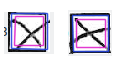
\includegraphics[width=2cm]{checkbox_good.png}


\end{center}
\vspace{1ex}
\vfill
\pagebreak
%%% fin de l'en-tête

\restituegroupe{groupes}


\AMCassociation{\id}

	  } % End \exemplaire{1}{%
} % End \newcommand{\sujet}{


%%%%§§§§§§§§§§§§§§§§§§§§§§§§§§§§§§§§§
\newcommand{\allq}{}

\begin{document}
%%%Options
\AMCrandomseed{10}

\def\AMCformQuestion#1{{\sc Question #1 :}}

\setdefaultgroupmode{withoutreplacement}
%%% Fin Options

%%% elements

\element{generalites}{
  \begin{questionmult}{gen1}
    Les humains ont besoin d'énergie pour~:
    \begin{reponses}
      \bonne{Cuisiner}
      \bonne{Se déplacer}
      \bonne{S'éclairer}
      \mauvaise{Les humains n'ont pas besoin d'énergie}
    \end{reponses}
  \end{questionmult}
}

\element{generalites}{
  \begin{questionmult}{gen2}
    Les humains ont besoin d'énergie pour~:
    \begin{reponses}
      \bonne{Se nourrir}
      \bonne{Se chauffer}
      \bonne{Voyager}
      \mauvaise{Les humains n'ont pas besoin d'énergie}
    \end{reponses}
  \end{questionmult}
}

\element{sources}{
  \begin{questionmult}{source1}
    Les énergies exploités par l'humanité~:
    \begin{reponses}
      \bonne{Se trouvent dans des sources d'énergies}
      \bonne{Se chauffer}
      \bonne{Voyager}
      \mauvaise{Surgissent spontanément}
    \end{reponses}
  \end{questionmult}
}

\element{sources}{
  \begin{questionmult}{source2}
    Une source d'énergie, c'est~:
    \begin{reponses}
      \bonne{Un phénomène naturel}
      \bonne{Exploitée par les humains pour en tirer de l'énergie}
      \mauvaise{Une passion qui anime l'humanité}
      \mauvaise{Une eau vivifiante qui jaillit d'une montagne}
    \end{reponses}
  \end{questionmult}
}

\element{carbone}{
  \begin{questionmult}{carb1}
    Coche les sources d'énergie carbonées~:
    \begin{reponses}
      \FPeval\ySeed{trunc(random*1000,0)}
      \input{"|./genexo.py --seed \ySeed~ --mode CARB1 --level 0 --qref toto \allq"}
    \end{reponses}
  \end{questionmult}
}

\element{carbone}{
  \begin{questionmult}{carb2}
    Les sources d'énergie carbonées~:
    \begin{reponses}
      \FPeval\ySeed{trunc(random*1000,0)}
      \input{"|./genexo.py --seed \ySeed~ --mode CARB2 --level 0 --qref toto \allq"}
    \end{reponses}
  \end{questionmult}
}

\FPeval\ySeed{trunc(random*1000,0)}
\input{"|./genexo.py --seed \ySeed~ --mode FNR --level 0 --qref toto \allq"}

\FPeval\ySeed{trunc(random*1000,0)}
\input{"|./genexo.py --seed \ySeed~ --mode FSNR --level 0 --qref toto \allq"}


\element{enrn}{
  \begin{questionmult}{nrrn}
    Coche les sources d'énergie renouvelables dans la liste~:
    \begin{reponses}
      \FPeval\ySeed{trunc(random*1000,0)}
      \input{"|./genexo.py --seed \ySeed~ --mode FRNR --level 0 --qref toto \allq"}
    \end{reponses}
  \end{questionmult}
}


%%%% fin des elements

\element{groupes}{
\section{Généralités}
\restituegroupe[1]{generalites}

\section{Énergies carbonées}
\begin{multicols}{2}
\restituegroupe{carbone}
\end{multicols}

\section{Sources et formes d'énergies}
\begin{multicols}{2}
\restituegroupe[8]{autofnr}
\restituegroupe[8]{autofsnr}
\restituegroupe{enrn}
\end{multicols}

\section{Pour aller plus loin}
\emph{Ce problème est plus difficile et rapporte moins de points, ne le faire que lorsque le reste est terminé, c'est un bonus!}

\subsection{En quoi les énergies carbonées sont-elles un problème pour l'avenir de l'humanité~?}
\begin{EnvQuadrillage}[NbCarreaux=21x6,Grille=Seyes,Marge=1]
\end{EnvQuadrillage}

\subsection{Quels problèmes résout l'énergie nucléaire parmi ceux soulevés plus haut~? Lesquels ne résout-elle pas~?}
\begin{EnvQuadrillage}[NbCarreaux=21x6,Grille=Seyes,Marge=1]
\end{EnvQuadrillage}

\subsection{En quoi les énergies renouvelables résolvent'elles ces problèmes~? Quels en sont cependant les inconvénients~?}
\begin{EnvQuadrillage}[NbCarreaux=21x6,Grille=Seyes,Marge=1]
\end{EnvQuadrillage}


\AMCcleardoublepage
}

\csvreader[head to column names]{liste.csv}{}{\sujet}

\end{document}
